\documentclass[./thesis.tex]{subfiles}

\begin{document}
\label{chap:APPLICATIONS}

In this chapter, we present applications that were made possible thanks by
the optimized CIPSI implementation presented in this thesis, and the hybrid
stochastic-deterministic algorithm. 
We first present a difficult benchmark of excited states, and then the use
of CIPSI wave functions for quantum Monte Carlo calculations.

\section{Excited states benchmark}

On figure~\ref{fig:energy_pt2}, one can see that both $\Evar$ and $\Evar+\EPT$
converge to the FCI energy when the number of determinants increases. A
convenient extrapolation introduced by Holmes~\textit{et al}\cite{Holmes_2017} is $\Evar$ as a
function of $\EPT$. Indeed, at the FCI limit $\EPT=0$ and $\Evar=\EFCI$.  Such
an extrapolation was used to estimate the FCI energies of the ground and
excited states of the molecules of the benchmark.

Another important point is to obtain a balanced description of both states,
such that the errors due to the approximations cancel nicely when looking at
energy differences. A way to achieve this goal is to select determinants for all
states simultaneously in a state-averaged fashion. Here, our selection criterion
for the external determinants was to take the maximum of the contribution
$\epsilon_\alpha$ among all the considered states.

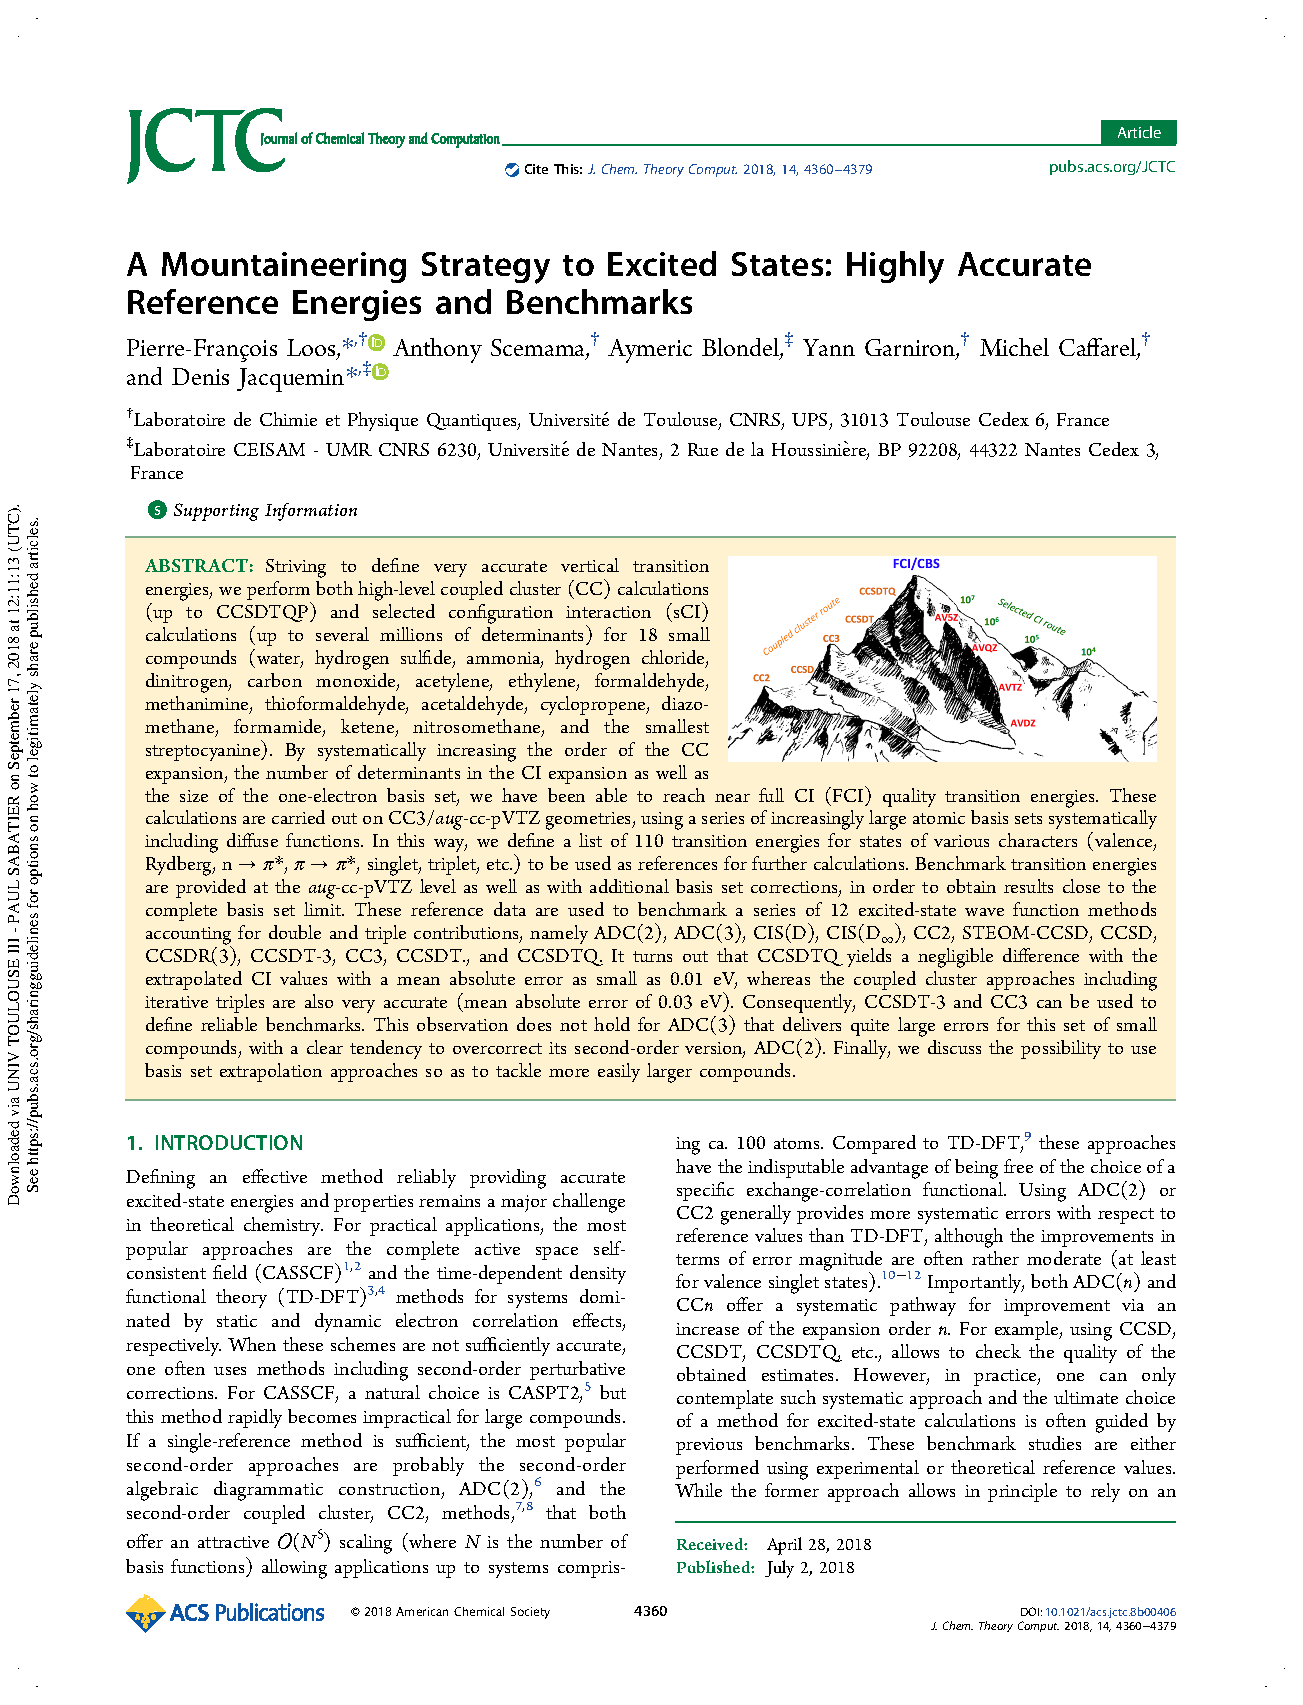
\includepdf[page=1-]{article_mountain}

\section{Application to QMC : the Fe--S molecule}


\newcommand{\rn}{\mathbf{r}_1,\dots,\mathbf{r}_N}
\newcommand{\drn}{\text{d}\mathbf{r}_1\,\dots\,\text{d}\mathbf{r}_N}
In a diffusion quantum Monte Carlo calculation (DMC), a trial wave function
$\Psi$ is required. One is able to compute
\begin{align}
  \EDMC = \frac{\Hij{\Phi^{\text{FN}}}{\Psi}}{\braket{\Phi^{\text{FN}}}{\Psi}} & = 
  \frac{\int \Phi^{\text{FN}}(\rn) {\hat H}\Psi(\rn) \drn}{\int \Phi^{\text{FN}}(\rn)\Psi(\rn) \drn} \\
  & = \frac{\int \Phi^{\text{FN}}(\rn)\Psi(\rn) \frac{{\hat H}\Psi(\rn)}{\Psi(\rn)} \drn}{\int \Phi^{\text{FN}}(\rn)\Psi(\rn) \drn} 
\end{align}
as a stochastic average with the $3N$-dimensional density $\Psi \times \Phi^{\text{FN}}$:
\begin{equation}
  \EDMC = \left \langle \frac{{\hat H}\Psi(\rn)}{\Psi(\rn)} \right \rangle_{\Psi \times \Phi^{\text{FN}}}.
\end{equation}
$\Phi^{\text{FN}}$ is an improved wave function of the form
\begin{equation}
\Phi^{\text{FN}}(\rn)  = \Psi(\rn) \times w (\rn)
\end{equation}
where $w$ is a non-negative function, given by
\begin{equation}
w(\mathbf{R}) = \lim_{t \rightarrow \infty} \exp \qty( \int_0^t \text{d}t \frac{{\hat H}\Psi(\mathbf{R}(t))}{\Psi(\mathbf{R}(t))} ).
\end{equation}
This expression can't be computed exactly, but it can be sampled with a diffusion
process with drift and branching.\cite{Hammond_1994}

The non-negativity constraint of $w$ implies that the nodal
hyper-surfaces of $\Phi^{\text{FN}}$ coincide with those of $\Psi$, but not necessarily with
those of the exact wave function. Hence, the Diffusion Monte Carlo (DMC) method
suffers from the so-called \emph{fixed-node approximation}. But if the trial wave
function has nodes which coincide with those of the exact wave function, the
exact energy is obtained.

There is no way to improve the nodes of the wave function by minimizing directly $\EDMC$.
However, it has recently been shown\cite{Caffarel_2016} that for each atomic basis
set there was an $\EDMC$ associated with the FCI wave function, and increasing the
size of the basis set enabled a smooth extrapolation to the exact energy.
Hence, one expects that computing DMC energy differences with FCI wave functions will
show an efficient compensation of errors.

In this work, we have introduced an extrapolation scheme, $\EDMC$ as a function
of $\EPT$ to estimate the $\EDMC$ we would have obtained if the trial wave
function was a FCI wave function. We have applied this scheme to the difficult
case of the Fe--S molecule, for which the nature of the ground state in not
clear. Two states of different symmetries, $^5\Sigma$ and $^5\Delta$ are very
close in energy, and the main methods of quantum chemistry disagree.
State-of-the art QMC calculations were giving the $^5\Delta$ state
as the ground state,\cite{Haghighi_Mood_2017} and our results agree with these
conclusions.


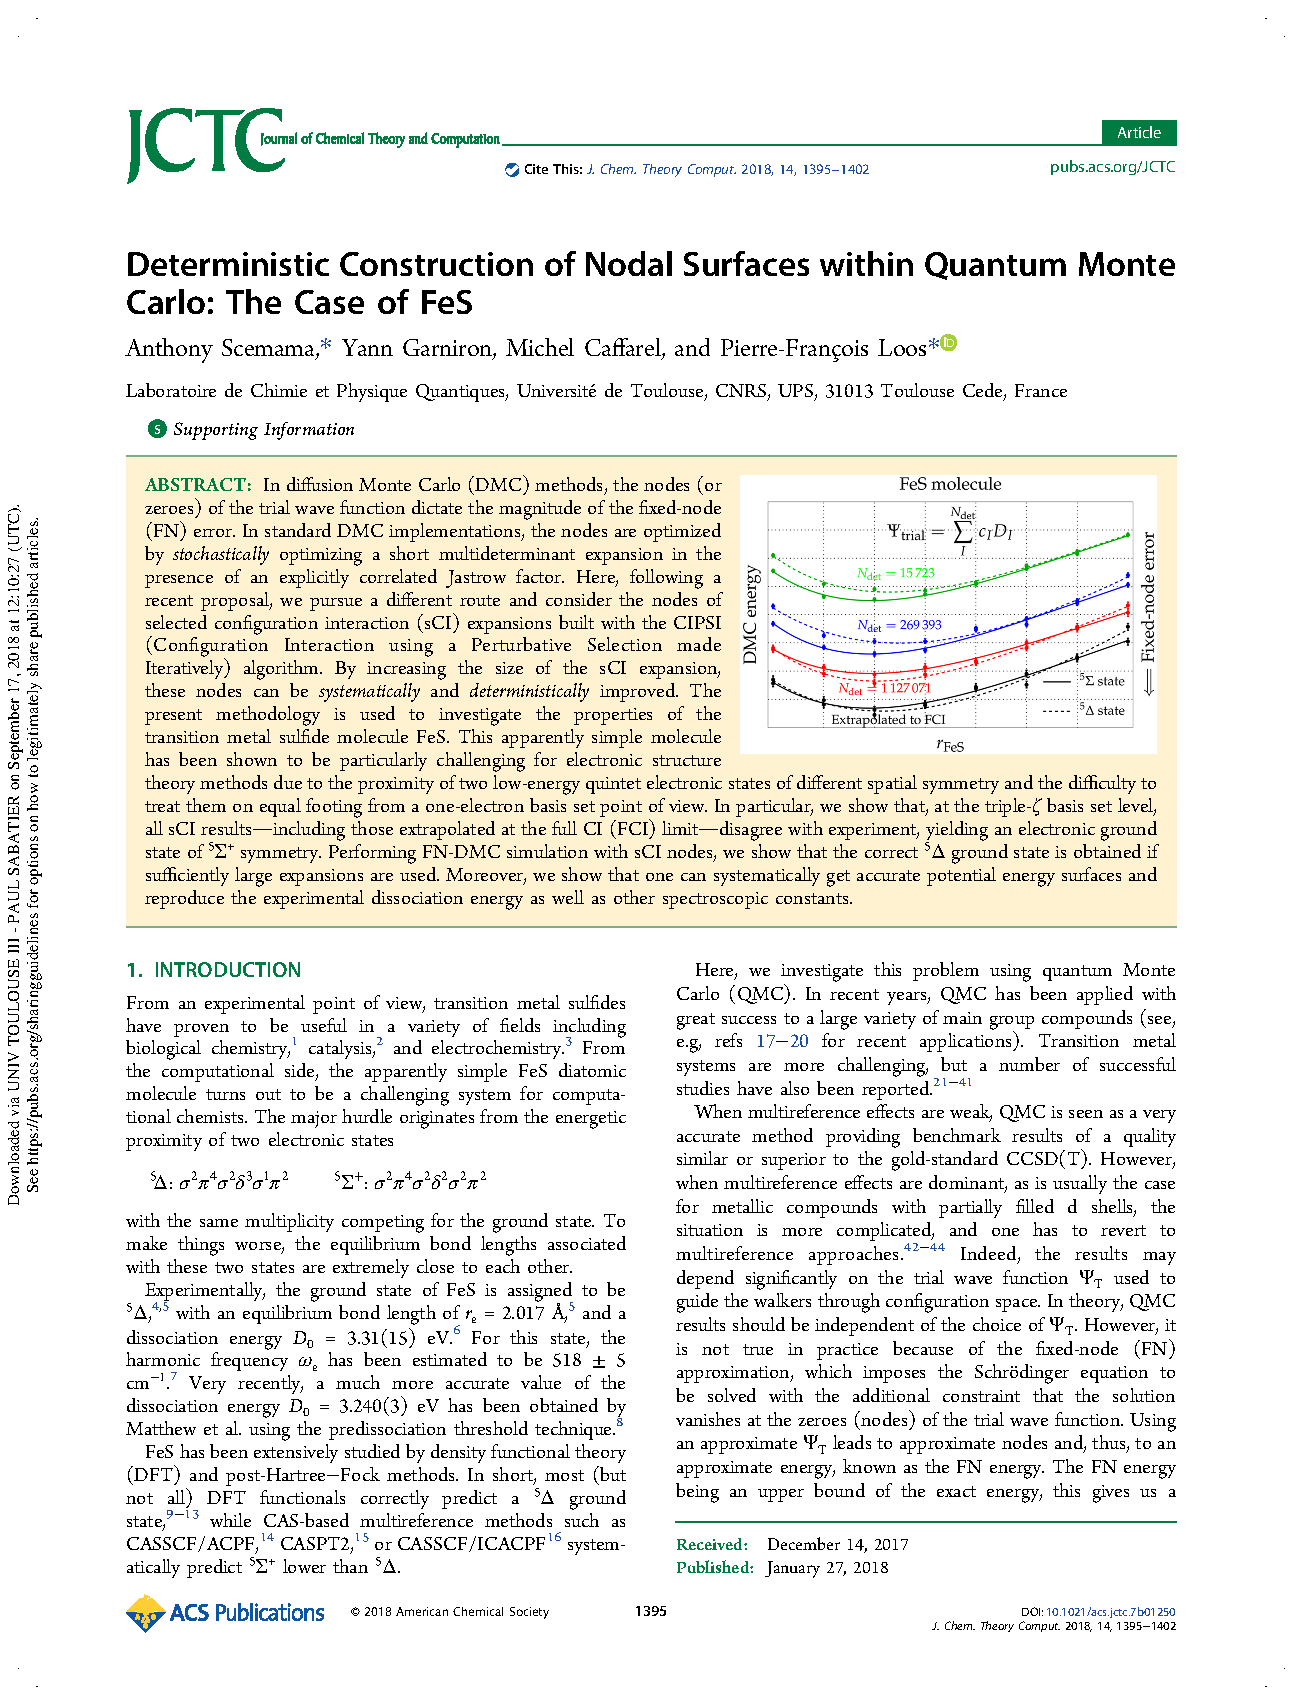
\includepdf[page=1-]{article_fes}

\end{document}
